% \documentclass[conference]{IEEEtran}
\documentclass[conference,compsoc]{IEEEtran}
% \documentclass[journal]{IEEEtran}
% \documentclass[10pt,journal,compsoc]{IEEEtran}
% \documentclass[journal,comsoc]{IEEEtran}
% \documentclass[journal,transmag]{IEEEtran}

\usepackage[utf8]{inputenc}
\usepackage[T1]{fontenc}
\usepackage[ngerman]{babel}
\usepackage{ifpdf}

\ifCLASSOPTIONcompsoc
  % \usepackage[nocompress]{cite}
  \usepackage[numbers,sort]{natbib}
\else
  \usepackage{cite}
\fi

\ifCLASSINFOpdf
  \usepackage[pdftex]{graphicx}
  \graphicspath{{../pdf/}{../jpeg/}}
  \DeclareGraphicsExtensions{.pdf,.jpeg,.png}
\else
  \usepackage[dvips]{graphicx}
  \graphicspath{{../eps/}}
  \DeclareGraphicsExtensions{.eps}
\fi

\usepackage{amsmath}
\usepackage{algorithmic}
\usepackage{array}

\ifCLASSOPTIONcompsoc
  \usepackage[caption=false,font=footnotesize,labelfont=sf,textfont=sf]{subfig}
\else
  \usepackage[caption=false,font=footnotesize]{subfig}
\fi

\usepackage{stfloats}
\usepackage{float}
\usepackage{url}

\hyphenation{op-tical net-works semi-conduc-tor}

\begin{document}
\title{Heiligt der Zweck die Mittel? - Wie werden Entscheidungen beim autonomen Fahren getroffen}

\author{
  \IEEEauthorblockN{Christoph Stach}
  \IEEEauthorblockA{
    Hochschule für Technik und Wirtschaft Berlin\\
    Fachbereich 4 - Angewandte Informatik\\
    s0555912@htw-berlin.de
  }
}

\maketitle

\begin{abstract}
    Autonomes Fahren ist ein noch relativ junges Forschungsfeld. Neue technologische Fortschritte machen es möglich, dass sich Fahrzeuge gänzlich ohne oder nur mit minimaler menschlicher Überwachung eigenständig auf Straßen oder in dafür vorgesehen Umgebungen bewegen können. Doch welche Gefahren bestehen beim autonomen Fahren und wer entscheidet in auftretenden Ernstfällen über den Ausgang einer Extremsituation? Das sind u. a. Fragen mit denen sich derzeit Wissenschaft und Gesellschaft gleichermaßen intensiv beschäftigten. Mit dieser Arbeit möchte der Author einen kurzen allgemeinen Überblick über das Themengebiet geben, z. B. welche Technologien zum Einsatz kommen, und versuchen, speziell das Treffen moralischer Entscheidungen in Extremsituation beim autonomen Fahren in der EU getroffen werden.
\end{abstract}
\section{Einleitung}

Heutzutage wird der Großteil der Fahrzeuge auf unseren Straßen durch Menschen gesteuert. Doch das könnte sich bald ändern. Schon jetzt unterstützen Fahrassistenzsysteme die Fahrer und warnen unter Umständen in Gefahrensituationen.

Das Forschungsfeld des autonomen Fahrens besteht aus unterschiedliche Teilgebiete. In diesem Artikel wird  zwischen dem rein technischen Bereich und dem sozial-technischen Bereich unterschieden. Technologischen Forschungen beziehen sich auf Hardware, z.B. unterschiedliche Sensoren, und Software, z.B. Algorithmen und Assistenzsysteme, die benötigt werden um ein autonom fahrendes Fahrzeug zu realisieren. Der sozial-technische Bereich umfasst die Auswirkungen auf die Gesellschaft und das Vertrauen in die neuartige Technologie. Die Aspekte die durch autonomes Fahren entstehen werden versucht durch Gesetzgeber mit Richtlinien zu regulieren und Verfahren zu standardisieren. Dadurch entsteht zur Zeit ein internationaler Wettlauf um die Vorherrschaft in diesem Gebiet.

In dieser Arbeit gehen ich zuerst in \ref{sec:verwandte-literatur} auf  verwandte Arbeiten mit dem Thema ein. Ich stelle die unterschiedlichen wissenschaftlichen Arbeiten, die sich mit der Internetseite \textit{The Moral Machine}\footnote{\url{http://moralmachine.mit.edu/}} beschäftigen, vor. Danach beschäftige ich mich mit den wesentlichen Definitionen und Technologien in \ref{sec:definitionen-und-technologie}, die in autonomen Fahrzeugen zum Einsatz kommen, ein. Schließlich rege ich eine ethische Diskussion in \ref{sec:diskussion} an und begründe meine persönlichen Gedankengänge in einem Fazit in \ref{sec:fazit}.
\section{Verwandte Literatur}
\label{sec:verwandte-literatur}

Die Arbeit bezieht sich auf die Fachschriften der Internetseite \textit{Moral Machine Website}. Des weiteren wird unterschiedliche Grundlagenliteratur, die sich mit allgemeinen Begriffen und Technologien des autonomen Fahrens beschäftigt, vorgestellt.\\

\citeauthor{roadblocks} identifizieren in ihrer wissenschaftlichen Publikation \textbf{Psychological roadblocks to the adoption of self-driving vehicles \cite{roadblocks}} unterschiedliche Dilemmas und auftretende Herausforderungen, deren sich die Gesellschaft stellen muss. Entscheidungsträger werden Richtlinien für diese Dilemmas finden müssen die gleichermaßen von der Gesellschaft akzeptiert werden müssen. Hierfür werden mögliche Lösungsvorschläge unterbreitet. 

Es wird identifiziert, dass die Mehrheit ein Verhalten von autonomen Fahrzeugen in Extremsituationen das dem Gesamtwohl zu gute kommt bevorzugen würde. Kaufen würden Personen jedoch Fahrzeuge die Ihnen selbst möglichst hohe Sicherheit gewährleisten. Diese beiden Fakten schließen sich gegenseitig aus.

Unausweichliche Unfälle autonomer Fahrzeuge werden zu Überreaktionen in der Gesellschaft führen, was die Einführung und Annahme verlangsamen oder lahm legen könnte.

Durch die Verwendung von Anwendungen aus dem Bereich des Maschinellen Lernens kann den Entscheidungsprozess, den autonome Fahrzeuge in bestimmten Situationen treffen, schlecht nachvollzogen werden. Das kann dazu führen, dass ein allgemeines Misstrauen gegenüber der Technologie entsteht.\\

In \textbf{The Social Dilemma of Autonomous Vehicles \cite{socialDilemma}} beschreiben \citeauthor{socialDilemma} die Ergebnisse einer Studie mit 1929 Teilnehmern. Diese wurden dazu befragt ob sie Fahrzeuge mit einem zweckorientierten Verhalten in Extremsituationen bevorzugen und ob sie diese kaufen würden. Damit baut die Publikation auf dem bereits identifizierten ethischen Dilemma aus \cite{roadblocks} auf. Über Auswertungen wird gezeigt, dass eine Regulierung von autonomen Fahrzeugen durch den Gesetzgeber zu einem zweckorientierten Verhalten die Einführung verlangsamen würde. Das hätte in der Gesamtheit mehr Todesfälle zur Folge als die frühe Einführung der Technologie, da langfristig mehr Unfälle durch Menschen verursacht werden als durch autonome Fahrzeuge. 90\% der Unfälle sind auf menschliche Fehler zurückzuführen.\\

Der Artikel \textbf{The Moral Machine experiment \cite{moralMachine}} von \citeauthor{moralMachine} untersucht die Daten, die über die eine weltweit verfügbare Umfrageplattform \textit{The Moral Machine} gesammelt wurden. Nutzer wurden nach dem moralisch besser vertretbaren Ausgang verschiedener unausweichlicher Unfallszenarien befragt. Zur Auswahl hat ein Nutzer jeweils zwei unterschiedliche Ausgänge in eine Extremsituationen. Bei den Ausgängen müssen entweder die Insassen des Fahrzeugs, oder Passenten auf der Straße sterben. In den Szenarien werden auf der Straße und im Fahrzeug jeweils unterschiedliche Personengruppen abgebildet. Jedes Unfallszenarium stellt dabei ein ethisches Dilemma dar. Es wurden unterschiedliche Statistiken erhoben auf die in dieser Arbeit referenziert wird. Außerdem über Beobachtungen ein Unterschied in der moralischen Bewertung der Unfallszenarien in verschiedenen Kulturkreisen identifiziert. Es wird dabei wesentlich zwischen westlichem, südlichem und östlichem Kulturkreis unterschieden. Gesamtheitlich wurde beobachtet, dass es starke Präferenzen der Befragten zum \textit{Retten von Menschen (gegenüber Tieren)}, zum \textit{Retten von vielen Leben (gegenüber weniger Leben)} und zum \textit{Retten von jungen Menschen (gegenüber alten Menschen)} gibt. Zum Zeitpunkt der Erstellung des Artikels, \citeyear{moralMachine}, wurden 39,61 Millionen Entscheidungen aus 233 Ländern weltweit gesammelt. \\

\textbf{A Voting-Based System for Ethical Decision Making \cite{votingBasedSystem}}, verfasst von \citeauthor{votingBasedSystem}, schlägt einen Algorithmen, mit dem ethische Entscheidungen in Extremsituationen getroffen werden können, vor. Es handelt sich dabei auf einen technischen Algorithmus, der anhand der Daten die von \textit{The Moral Machine} gesammelt wurden, Entscheidungen treffen kann. Der Algorithmus wertet die Ergebnisse aller Teilnehmern der Plattform aus, führt diese zusammen und ist in der Lage  \textit{swap-dominance efficient} das finden von Alternativen zu erlernen. Methoden des Maschinellen Lernens werden verwendet und der trainierte Algorithmus ist in der Lage, die ethisch am besten zu akzeptierenden Ausgänge für eine Extremsituationen aus einer Menge von Alternativen zu finden.\\

Neben der Literatur von \textit{The Moral Machine} baut dieses Arbeit auf unterschiedlichen Grundlagewerken zum Thema des autonomen Fahrens auf. Der vom \citeauthor{smith2015automated} veröffentlichte Bericht \textbf{Automated and
autonomous driving: regulation under uncertainty \cite{smith2015automated}} beschreibt allgemeine Technologien und Terminologien der Domäne.\\

Außerdem werden die SAE-Level des Standard \textbf{Taxonomy and Definitions for Terms Related to Driving Automation Systems for On-Road Motor Vehicles \cite{standardSAE}} der \citeauthor{standardSAE} vorgestellt (siehe. \ref{ssec:sae-level}).\\


\section{Definitionen und Technologie}
\label{sec:definitionen-und-technologie}

In diesem Teil werden die grundlegenden Technologien und Definitionen beschrieben, die zum Verständnis von autonomen Fahren wichtig sind.

\subsection{SAE-Level}
\label{ssec:sae-level}

Die SAE-Level \cite{standardSAE} beschreiben den Grad an Autonomie bei Fahrzeugen. Sie werden dabei in sechs unterschiedliche Stufen eingeteilt und wurden von der \citeauthor{standardSAE} definiert.\\

\subsubsection*{Level 0 - Keine Automatisierung} Der Fahrer übernimmt die volle Kontrolle über das Fahrzeug.

\subsubsection*{Level 1 - Fahrassistenz} Der Fahrer wird durch einen einzelnen Fahrassistenten, z.B. Tempomat, Spurhalteassistent oder Bremsassistent, unterstützt, behält jedoch die volle Kontrolle über das Fahrzeug.

\subsubsection*{Level 2 - Partielle Automatisierung} Der Fahrer wird durch mehrere Fahrassistenten unterstützt and hat immer die Kontrolle über das Fahrzeug.
    
\subsubsection*{Level 3 - Bedingte Automatisierung} Das Fahrzeug ist in der Lage, die Umgebung zu erkennen und eigenständig bestimmte Fahrsituationen zu meistern. Ein aufmerksamer Fahrer ist trotzdem erforderlich, um unter Umständen einzuschreiten.

\subsubsection*{Level 4 - Hohe Automatisierung} Das Fahrzeug kann eigenständig in den meisten Fahrumgebungen manövrieren. Es erkennt Fehlentscheidungen und kann auf diese reagieren. Menschliches Einschreiten ist, wenn gewünscht, möglich.

\subsubsection*{Level 5 - Volle Automatisierung} Das Fahrzeug kann in allen Umgebungen, zu jeder Zeit und in jeder Situation komplett eigenständig fahren.

\subsection{Sensoren}

In autonomen Fahrzeugen kommen unterschiedliche Arten von Sensoren zum Einsatz. 
Dazu gehören Kameras, Radars, spezielle Laserscanner und Ultraschallsensoren.\\

\begin{figure}[H]
    \centering
    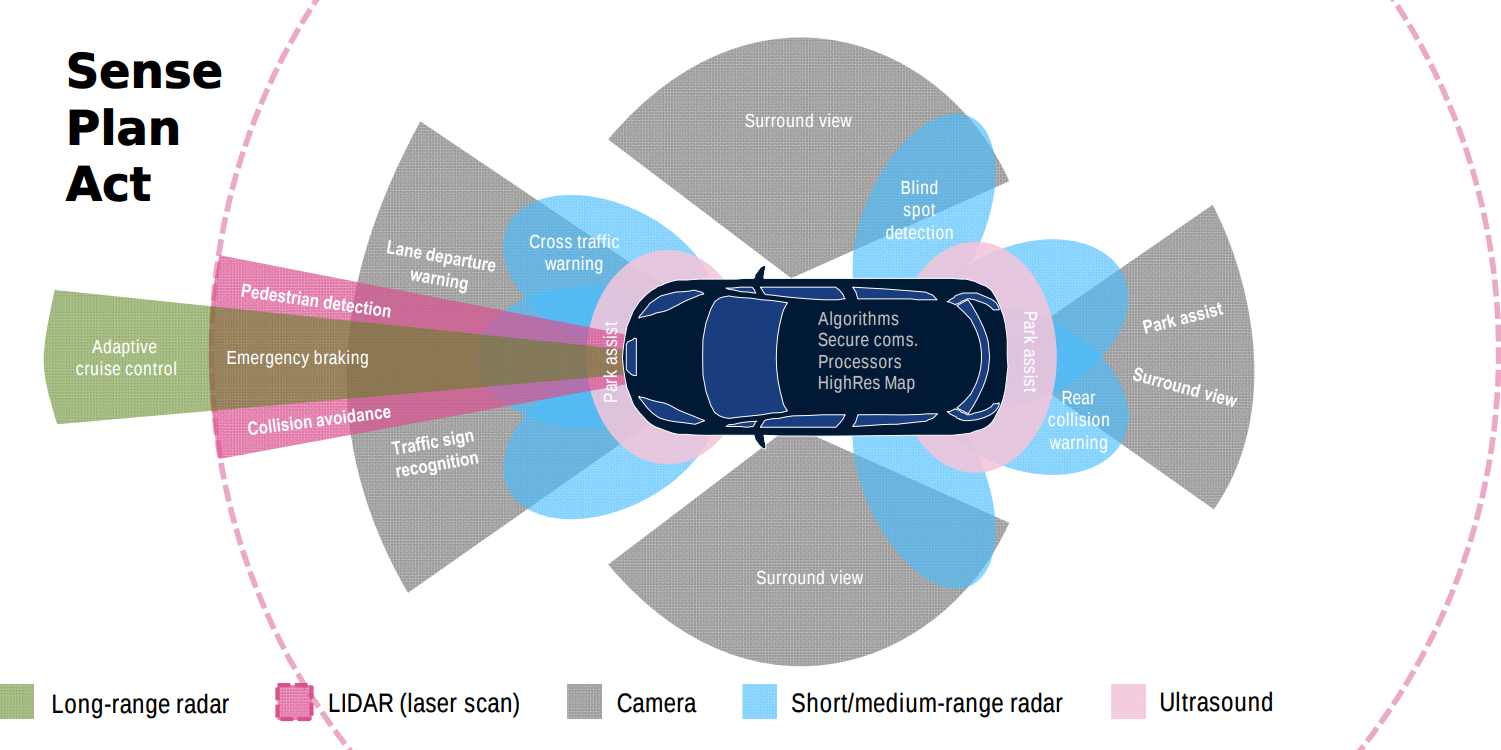
\includegraphics[width=.485\textwidth]{resources/images/sensors.png}
    \caption{Sensoren eines autonomen Fahrzeuges \cite{smith2015automated}}
\end{figure}

Kameras können rund um das Fahrzeug montiert werden und ermöglichen dem Fahrzeug somit eine vollumfängliche Sicht auf das Verkehrsgeschehen. Ein Vorteil gegenüber einem menschlichen Fahrer ist, dass auch tote Winkel mit Kameras überwacht werden können. Die Blickwinkel der Kameras lassen jedoch u. U. die Entfernung zu erkannten Objekten schlecht einschätzen.\\

Dazu wird die LIDAR-Technologie \cite{himmelsbach2008lidar} verwendet. LIDAR steht für \textit{Light Detection and Ranging}. Es handelt sich um eine Umgebungsüberwachungstechnik, die mit Hilfe eines Lasers Objekte in der Nähe bestrahlt und die Reflexion mit einem Sensor misst. So kann die Entfernung zu den Objekten berechnet werden.\\

Radar-Systeme \cite{introductionToRadarSystems} funktionieren ähnlich wie LIDAR-Systeme. Anstatt von Lichtwellen werden Radiowellen eingesetzt. Objekte in der Umgebung erzeugen ein Echo, welches von einem Sensor empfangen wird. Somit ist ein Radar-System in der Lage, die Distanz, Position und Geschwindigkeit von Objekten zu berechnen.\\

Neben Radar- und LIDAR-Systemen können weitere Sensoren in autonomen Fahrzeugen zum Einsatz kommen. Hierzu zählen beispielsweise Ultraschall und Infrarot.
Ultraschall wird auch in der Natur von Fledermäusen eingesetzt. Es funktioniert ähnlich wie ein Radar, hat jedoch eine geringere Reichweite und ist somit besser geeignet, um Objekte in der direkten Umgebung des Fahrzeuges zu erkennen.\\

Mit Hilfe der verschiedenen Sensorsystemen ist man in der Lage, ein komplettes 3D-Abbild der Umgebung zu erstellen. Damit hat ein autonomes Fahrzeug einen entscheidenden Vorteil gegenüber einem Menschen, der Objekte außerhalb seines Sichtfeldes nicht identifizieren kann.\\

\subsection{Vehicular Ad-hoc Network}

Fahrzeuge vernetzen sich mit anderen Fahrzeugen und der Infrastruktur über ein \textit{VANET}. Das \textit{VANET} ist eine Abwandlung des \textit{MANETs (Mobile Ad-hoc Network)}. 

\begin{figure}[H]
    \centering
    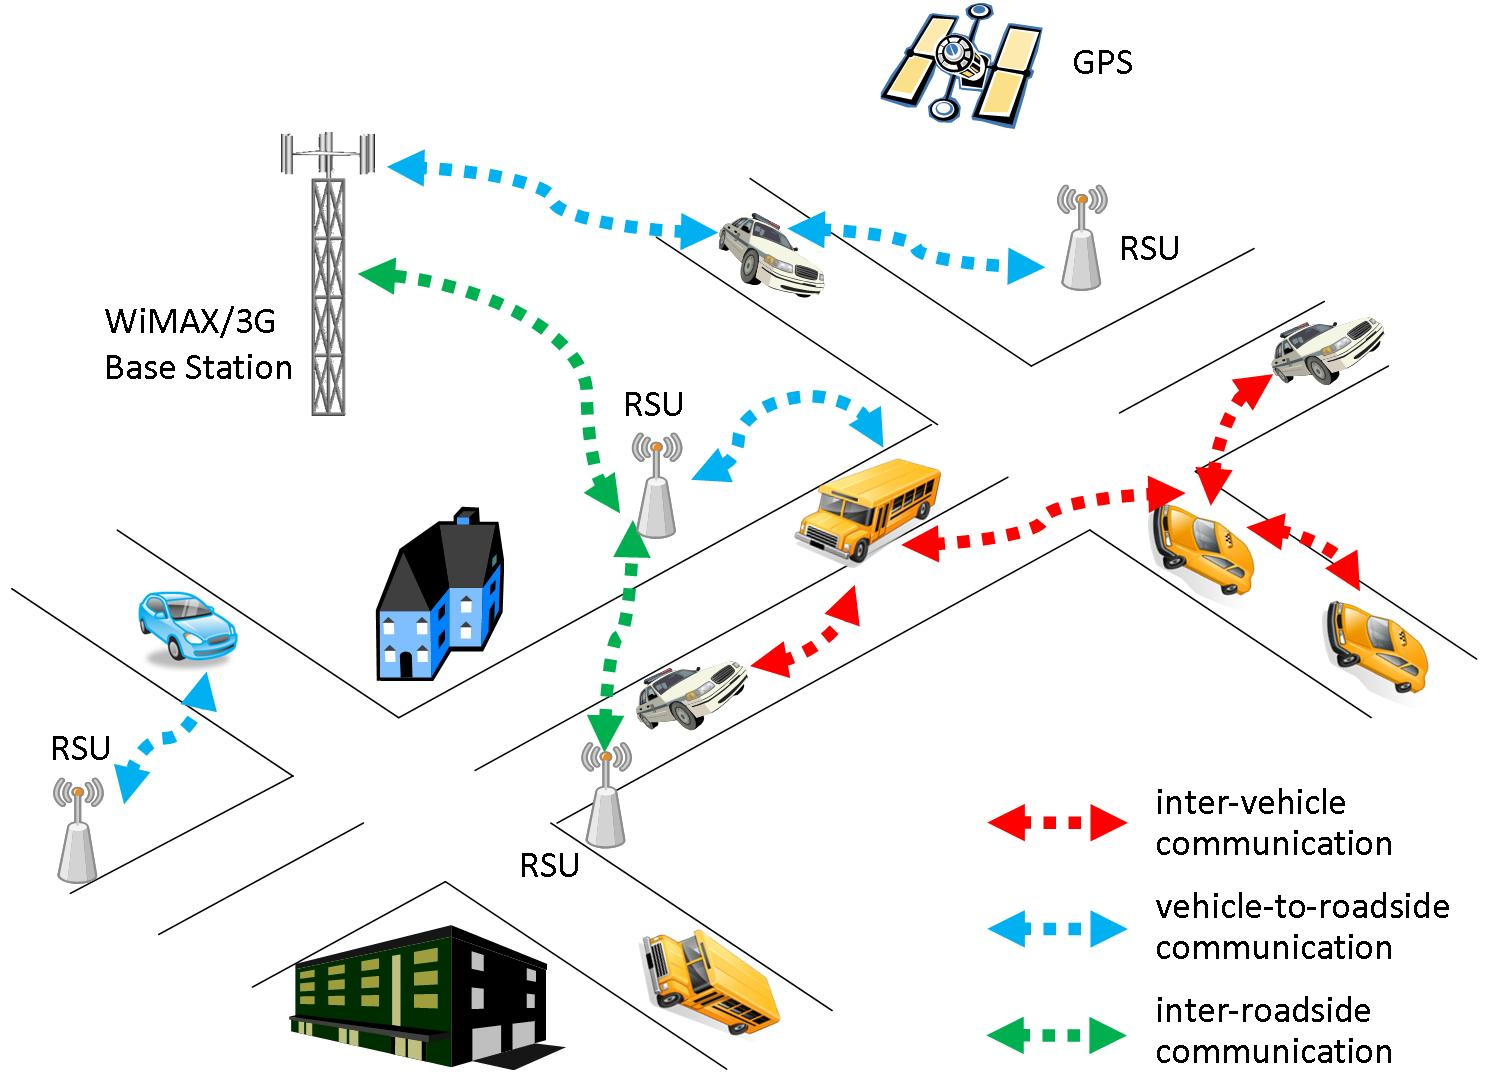
\includegraphics[width=.485\textwidth]{resources/images/vanet.jpg}
    \caption{Übersichtsgrafik eines VANETs \cite{vanet}}
\end{figure}

Durch die Verwendung von VANETs können Fahrzeuge untereinander und mit der Infrastruktur kommunizieren. Somit kann eine Ampel ihren aktuellen Status an das passierende Fahrzeug senden und ihm mitteilen, ob sie rot, gelb oder grün leuchtet. Das Fahrzeug kann darauf hin eine Entscheidung treffen, wie es sich verhalten soll. Eine weitere Anwendungsmöglichkeit ist beispielsweise die Stauerkennung. Fahrzeuge können sich untereinander austauschen, ob sie sich in einem Stau befinden. So können andere Verkehrsteilnehmer gewarnt und entsprechende Stauabschnitte automatisch umfahren werden.

\subsection{Software}

In autonomen Fahrzeugen kommt unterschiedliche Software zum Einsatz. Algorithmen aggregieren die Daten der Sensoren und treffen Entscheidungen über den Fahrtverlauf. Außerdem übernimmt Software die Kommunikation zu anderen Verkehrsteilnehmern und der Infrastruktur. Damit sich die Fahrzeuge besser orientieren können, werden hochauflösende Karten eingesetzt.
\section{Diskussion}
\label{sec:diskussion}

Die Arbeit behandelt Fahrzeuge des SAE-Levels 4 und 5. Denn nur diese sind in der Lage ohne Supervision eines Fahrers sich im Straßenverkehr zu bewegen. 

\subsection{Vorteile}

Autonomes Fahren bringt viele Vorteile mit sich. Durch die unterschiedlichen Sensoren kann ein weitaus größeres Sichtfeld erzeugt werden, als es mit dem menschlichen Auge möglich ist. Software trifft Entscheidung binnen Millisekunden und kann akkurate Berechnungen über den Fahrtverlauf durchführen. 
Da es sich bei 90\% der Unfälle um menschliches Fehlverhalten handelt kann die die Einführung autonomer Fahrzeuge die Unfallrate dementsprechend senken \cite{roadSafty}.\\

Durch die effiziente Kommunikation der Fahrzeuge untereinander können Staus vermieden werden. Der Verkehr würde sich besser auf unterschiedliche Teile des Verkehrsnetzes verteilen. Das verkürzt die Fahrzeiten. \\

Mit geteilten autonomen Fahrzeugen, die Teil der öffentlich Verkehrsmittel werden, kann die Anzahl der Fahrzeuge auf den Straßen verringert werden. Die meiste Zeit stehen private Fahrzeuge auf Parkplätzen. Die Parkplatzsuche würde entfallen, was gerade in Großstädten ein bekanntes Problem ist. Eine Studie der Berryls Strategy Advisor zeigt das der Einsatz von 18.000 Robotertaxis den gesamten privaten Verkehr sowie 20\% des Pendlerverkehrs der Stadt München abdecken kann \cite{advisors2017simulation}.\\

Verkürzte Fahrtzeiten und weniger Fahrzeuge auf den Straßen wirkt sich positiv auf die Treibstoffemissionen aus. Somit würde der Einsatz von autonomen Fahrzeugen langfristig einen Beitrag zum Umweltschutz leisten.\\

\subsection{Herausforderung}

Die flächendeckende Einführungen von autonomen Fahrzeugen wird die Gesellschaft und auch Gesetzgeber vor Herausforderungen stellen. Zur Zeit existieren nur vage Richtlinien für das Testen und den Betrieb \cite{doi:10.1080/01441647.2018.1494640}. Fraglich ist auch wie sich autonome Fahrzeuge verhalten sollen, wenn sie Staatengrenzen überqueren. Gerade in Europa sind die meisten Grenzen offen und viele Menschen pendeln zwischen Ländern. Unterschiedliche Gesetzgebungen müssen bei der Entwicklung autonomer Fahrzeuge beachtet werden.\\

Gerade in Deutschland, wo ein Auto als Statussymbol gilt, wird sich die Einführung autonomer Fahrzeuge im privaten Sektor als schwierig erweisen. Außerdem sind Deutsche sehr misstrauisch gegenüber neuer Technologie [TODO Zitat von Studie]. Bis ein selbstfahrendes Auto von der Mehrheit der Bevölkerung akzeptiert wird, wird es eine Zeit dauern. Ähnliche Hürden wurden auch in der Publikation \cite{roadblocks} von \citeauthor{roadblocks} identifiziert.\\

Ein besonderes Augenmerk muss auf die Entscheidungsfindung in Extremsituation gelegt werden. Als Extremsituation wird eine Situation definiert in denen ein Unfall unausweichlich ist. Beispielsweise wäre das bei einem plötzlichen mechanischen Versagen der Bremsen der Fall. Fahrzeuge müssen in diesen Situation den akzeptabelsten Ausgang finden. In der nächsten Sektion \ref{ssec:entscheidungen-in-extremsituationen} wird gesondert diesen Spezialfall eingegangen. Die Studie \cite{socialDilemma} geht gesondert auf diese Thematik ein. Sie zeigt, dass unterschiedliches Implementierungsmethoden für die Entscheidungsfindung in Extremsituationen das Kaufverhalten und somit die Zeit bis autonome Fahrzeuge gesellschaftlich akzeptiert werden, beeinflussen. Das wird sich besonders bei einem technikskepsischen Volk, wie den Deutschen, negativ auf die Akzeptanzzeit auswirken. In \citeauthor{socialDilemma} wird ebenfalls gezeigt, dass die Regulierung durch Gesetzgeber diesen Prozess noch weiter verlangsamen kann.\\


\subsection{Entscheidungen in Extremsituationen}
\label{ssec:entscheidungen-in-extremsituationen}

Wie werden Entscheidungen autonomer Autos in Extremsituationen getroffen? Diese Frage beschäftigt Ethikwissenschaftler. Über die Internetseite \textit{The Moral Machine} wurden weltweit große Mengen von Daten erhoben. Besucher der Internetseite werden befragt welcher der ethisch besser zu akzeptierende Ausgang einer Extremsituation ist. Dabei muss der Teilnehmer der Befragung jeweils zwischen zwei Ausgängen wählen. Man hat die Wahl das Auto in eine Barriere fahren zu lassen und somit die Insassen zu töten oder Menschen, die rechtens oder auch unrechtens, die Ampel überqueren zu töten. Dabei werden einem verschiedene Szenarien mit unterschiedlichen Menschen als Insassen und Passanten gezeigt. Die gesammelten Daten stehen frei zur Verfügung.\\

Mit gesammelten Daten der Internetseite wurden umfassend ausgewertet, um zu sehen wie der allgemeine Status Quo der Gesellschaft zum Thema ethische Entscheidungsfindung in Extremsituation von autonomen Fahrzeugen ist. Eine Studie hat ergeben die meisten Entscheidung zu Gunsten vieler Personen, junger Personen und Menschen (auch Tiere werden in der \textit{Moral Machine} Internetseite gezeigt) gefallen sind. Jedoch gibt es kulturelle Unterschiede. Beispielsweise werden in östlichen Kulturen, wie in vielen Asiatischen Ländern, alte Menschen bevorzugt. Es wurden drei große Hauptgruppen gefunden die, die größten Meinungsunterschiede haben. Es handelt sich um die westliche, südliche und östliche Gruppierung \cite{moralMachine}.\\

% Hier weiter lesen!

Auf der Basis der gesammelten Daten wurde außerdem ein Algorithmus \cite{votingBasedSystem} entwickelt. Dieser ist in der Lage in Extremsituation Entscheidungen zu fällen. Es ist jedoch fraglich wie die Entscheidungen gefällt werden. Europa ist ein sehr diverser Kontinent mit vielen unterschiedlichen Kulturen, Religionen und Sprachen. Die Unterschiede in der Entscheidungsfindung fallen weitaus größer aus als beispielsweise in den komplett englischsprachigen USA. Laut der Studie befindet sich Frankreich in der südlichen Gruppieren, wobei sich Deutschland in der westlichen Gruppierung befindet. Das stellt Entscheidungsträger die Herausforderung ein einheitliches System zu finden was jedem Land gerecht wird.\\

Deswegen weisen die Autoren des Algorithmus, \citeauthor{votingBasedSystem}, darauf hin das die gesammelten Daten nicht komplett sein. Befindet man sich in einer Systemsituation mit seinem Fahrzeug ergeben sich mehr Optionen als das Fahrzeug in eine Barriere fahren zu lassen oder nicht einzugreifen. Außerdem kann es sein das sich geliebte Personen oder Verwandte mit im gleichen Fahrzeug befinden. Das hätte Einfluss auf die Entscheidungsfindung bei Menschen. Das sind Faktoren die bei Sammeln der Daten mit \textit{The Moral Machine} nicht berücksichtigt worden sind.\\

Das Europäische Parlament hat im April 2019 die \textit{Ethik-Leitlinien für eine Vertrauenswürde KI} für den Umgang mit Systemen der Künstlichen Intelligenz veröffentlicht \cite{ec2019ethics}. Autonome Fahrzeuge setzen auf viele Systeme der künstlichen Intelligenz. Beispiele hier für sind die Bilderkennung und Objekterkennen oder die Algorithmen über die Entscheidungsfindung. Bei autonomen Fahrzeugen kommt es jedoch zu einem Konflikt mit diesen Leitlinien. Beispielsweise mit Leitlinie Nr. 1, \textit{Vorrang menschlichen Handelns und menschliche Aufsicht}, die bei Fahrerlosen Autos des SAE-Levels 4 oder 5 nicht zutreffen würde. Die Autoren des Dokuments, die \citeauthor{ec2019ethics}, kommentieren jedoch das die Leitlinien nicht endgültig sind. Außerdem müssen diese für bestimmte Teilgebiete der KI angepasst werden und erweitert. Das Dokument ist außerdem in Bearbeitung und soll zukünftig als Grundlage für weitere Leitlinien dienen.\\
\section{Fazit}
\label{sec:fazit}

Der in \citeauthor{votingBasedSystem} vorgestellten Algorithmus deckt lediglich einen Bruchteil der moralischen Entscheidungsraums ab. Schutzbedürftige Gruppen, laut \cite{ec2019ethics}, werden vernachlässigt. Außerdem gestaltet sich die Einführung des Algorithmus innerhalb einer Zone mit vielen unterschiedliche Kulturen schwierig.\\

Durch das Fehlen von spezifischen Ethikleitfäden, zugeschnitten auf das Themengebiet des autonomen Fahrens, fällt es schwer genaue aussagen zu Treffen wie sich autonome Fahrzeuge moralisch in Extremsituationen verhalten sollen.\\

Wie sich die Zukunft entwickeln wird, wird sich zeigen. Jedoch kann abschließen gesagt werden, das im Bereich der autonomen Fahrens noch viel Arbeit zu tätigen ist. Ethische Fragen sind nur bedingt geklärt konkrete Lösungen existieren noch nicht.


% \bibliographystyle{IEEEtranN-de}
% \bibliography{IEEEabrv,references/scientific,references/online,references/images}
\printbibliography

\end{document}